\begin{pastexam}[label={px:ust-115-ee-ds-22}]{臺聯大電機類 115 學年度 第 22 題}
（單選；2 分）

\textbf{Height:} Assume that the height of a tree node is the number of edges on the longest path
from the node to a leaf. A leaf node will have a height of 0.\\
\textbf{Balance:} The balance of a binary tree node is defined as \textbf{the left child node's
height minus the right child node's height}. The balance of a leaf node is 0 (since the height of a
\textbf{NULL} child node is defined as -1).\\
\textbf{What is the height of the root of a Binary Search Tree (BST) after inserting 5, 3, 9, 2, 4,
7, 1, 6, 10, 8? The tree is empty initially}

(A)~3 \qquad (B)~4 \qquad (C)~5 \qquad (D)~6 \qquad (E)~7
\end{pastexam}

\begin{pastsoln}
答案是 (A)。

依序插入（資結書虛擬碼~9.6，每個新鍵值從根往下比，小往左、大往右，接在 \NIL 的位置）：
$5$ 是根；$3 < 5$ 往左；$9 > 5$ 往右；$2$：$< 5$、$< 3$，成為 $3$ 的左孩子；$4$：$< 5$、$> 3$，
成為 $3$ 的右孩子；$7$：$> 5$、$< 9$，成為 $9$ 的左孩子；$1$：成為 $2$ 的左孩子；$6$：$> 5$、
$< 9$、$< 7$，成為 $7$ 的左孩子；$10$：成為 $9$ 的右孩子；$8$：$> 5$、$< 9$、$> 7$，成為 $7$ 的
右孩子。
\begin{center}
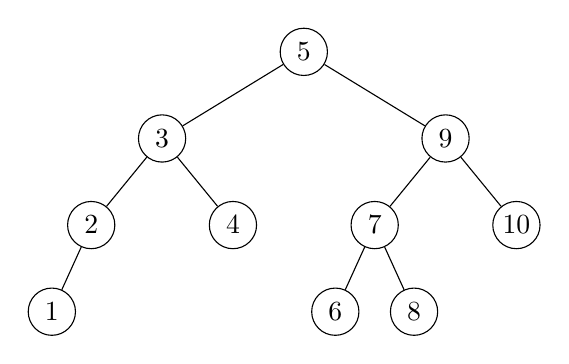
\begin{tikzpicture}[level distance=11mm, every node/.style={circle, draw, minimum size=6mm, inner sep=0pt},
  level 1/.style={sibling distance=36mm}, level 2/.style={sibling distance=18mm},
  level 3/.style={sibling distance=10mm}]
\node {5}
  child {node {3} child {node {2} child {node {1}} child[missing]} child {node {4}}}
  child {node {9} child {node {7} child {node {6}} child {node {8}}} child {node {10}}};
\end{tikzpicture}
\end{center}
高度用邊數算、葉子是 $0$。 由下往上：$1, 4, 6, 8, 10$ 是葉子，高度 $0$；$2$ 的高度是 $1$；
$7$ 的高度是 $1$；$3$ 的高度是 $1 + \max(1, 0) = 2$；$9$ 的高度是 $1 + \max(1, 0) = 2$；根 $5$ 的
高度是 $1 + \max(2, 2) = 3$。 最長的根到葉路徑是 $5 \to 3 \to 2 \to 1$（或 $5 \to 9 \to 7 \to 6$），
$3$ 條邊。

選項 (B)--(E) 都比 $3$ 大。 (B) $4$ 是用「節點數」算高度的結果（路徑上有 $4$ 個節點），題目明定
用邊數。 其餘更大的值不對應任何一種算法。
\end{pastsoln}
